%% The first command in your LaTeX source must be the \documentclass command.
%%
%% Options:
%% twocolumn : Two column layout.
%% hf: enable header and footer.
\documentclass[
% twocolumn,
% hf,
]{ceurart}

%%
%% One can fix some overfulls
\sloppy

%%
%% Minted listings support 
%% Need pygment <http://pygments.org/> <http://pypi.python.org/pypi/Pygments>
\usepackage{listings}
\lstset{upquote=true}

\usepackage{graphicx}

%% auto break lines
\lstset{breaklines=true}
\lstset{basicstyle=\ttfamily} 
%%
%% end of the preamble, start of the body of the document source.
\begin{document}

%%
%% Rights management information.
%% CC-BY is default license.
\copyrightyear{2022}
\copyrightclause{Copyright for this paper by its authors.
  Use permitted under Creative Commons License Attribution 4.0
  International (CC BY 4.0).}

%%
%% This command is for the conference information
\conference{Managing the Evolution and Preservation of the Data Web (MEPDaW 2022)}

%%
%% The "title" command
\title{Building materializable querying interfaces with the TREE hypermedia specification}

%%
%% The "author" command and its associated commands are used to define
%% the authors and their affiliations.
\author{Pieter Colpaert}[%
orcid=0000-0001-6917-2167,
email=pieter.colpaert@ugent.be,
url=https://pietercolpaert.be/#me,
]
\address{IDLab, Department of Electronics and Information Systems, Ghent University -- imec\\
Technologiepark-Zwijnaarde 122, 9052 Ghent, Belgium}


%%
%% The abstract is a short summary of the work to be presented in the
%% article.
\begin{abstract}
Ever since the Web was introduced to access representations of resources via URLs, Web developers have been coming up with ways to make available more specific HTTP responses via more complex URL patterns.
Complex URL patterns with features such as the SPARQL query language, GraphQL, OGC Web Feature Services, or free text queries, also come with limitations:
i) you can only query the data integrated on the machine you query,
ii) coding against a fixed protocol lowers potential evolvability,
iii) relying on dynamic server functionality raises challenges in long-term preservation, and
iv) sending the full query to a third party server lowers query privacy.
Linked Data Fragments puts forward the idea that there is a false dichotomy between solving the full query on the server of the data publisher and solving it fully on the infrastructure of the consumers:
when publishing data in fragments of triples in a dataset with a certain locality into an interlinked resource-structure, data consumers can speed up their own query processing.
In this paper, we build evolvable and preservable Web APIs using “materializable interfaces” with the TREE hypermedia specification.
For use cases such as route planning, full-text search, geospatial look-ups or replication and synchronization, we show how to build a fragmentation by qualifying the relation from one fragment to another.
This way, the TREE hypermedia specification helps to overcome the four drawbacks of URL-based query protocols.
The specification will be further developed as part of a W3C community group for which we are now seeking support.
\end{abstract}

%%
%% Keywords. The author(s) should pick words that accurately describe
%% the work being presented. Separate the keywords with commas.
\begin{keywords}
  TREE,
  Hypermedia,
  Linked Data Event Streams,
  Data publishing,
  RDF,
  Semantic Web,
  Linked Data Fragments
\end{keywords}

%%
%% This command processes the author and affiliation and title
%% information and builds the first part of the formatted document.
\maketitle

\section{Introduction}

The Web is a global information system that makes representations of resources addressable using URLs.
While the most visible use case to end-users is using URLs to address websites and their pages in their browser, developers also use exactly the same technique in what they call Web APIs to share data between user agents.
Just like a website, not all content or data that is managed through one server is exposed via only one resource.
Instead, a Web API is a resource structure that exposes one or more views over the collection of data.

\texttt{https://your-domain/your/resource/structure{?parameters}}

Depending on how tightly coupled the user-agent application and the Web API are, designing the resource structure of the Web API becomes more or less straightforward.
I.e. if there is only one app that needs the data the API exposes, and both are controlled by the same developer, the resource structure can be driven by exactly the user stories of the app itself.
However, if an unknown number of potential systems need to be able to reuse the data, such as it is the case when designing APIs for Open Data publishing, or resource structures within the Solid project\footnote{\url{https://solidproject.org/}}, it becomes guess-work on what API will work best.

The Linked Data Fragments (LDF) axis~\cite{verborgh_jws_2016} for building Web APIs describes two extremes: i) either the user agent downloads the full dataset and performs all processing on their infrastructure, ii) either the server creates an ad-hoc resource that gives precisely the data the user agent wants based on a query that is sent to the server.
Examples of the latter include the SPARQL protocol for querying RDF data, but equally as well, GraphQL, a full-text search API or a geospatial Web Feature Service (WFS).
These specifications allow almost any flexibility to be given to the user agent developer to formulate any possible query.
However, creating ad-hoc resources answering the full query on a server poses four important limitations:

\begin{description}
  \item[1. You are querying a closed world] You only query the data integrated on the machine you query. This will thus not be a good solution for cases in which you do not control the server you want to query: it could not have the features or data you need for your use case.
  \item[2. It is challenging to archive]
 Relying on dynamic server functionality raises challenges in long-term preservation.
 When the amount of different queries you can ask the server is infinite, what queries will you archive?
 \item[3. It is difficult to turn off or evolve an API once it has been made available]
 Coding against a purpose-built protocol lowers the potential evolvability of that API.
 Turning off this API in favour of a different specific Web API with ad-hoc resources built based on a specific language will require applications to be recoded towards that novel specification.
 \item[4. It leaks query privacy]
Sending the full query to a third party server shares the full questions your users are interested in to that server.
\end{description}

These two extremes are positioned as a false dichotomy by LDF.
If the user agent and the initial server can take up more responsibility in the query processing, then more options come to exist.
A dataset that is too big for one page can be \textit{fragmented} according to a certain property in the data, and therefore, by documenting the property, can help the user agent in pruning what fragments it needs to download in order to answer a certain query. 

The idea is further extended by Linked Data Event Streams (LDES)~\cite{ldes}.
LDES further reasons the ideal Web API on top of a dataset does not exist, as any type of fragmentation will introduce bias towards a specific use case.
Therefore, a dataset will be published through \textbf{multiple Web APIs} as illustrated in \cref{multiple-views}, and not just one, managed by multiple organizations using multiple Web servers.
LDES continues by then positioning that, if multiple views must become possible, that the first Web API a data publisher should build, is an event source, that focuses on keeping derived Web APIs in-sync with its authoritative source over the Web.

\begin{figure}
  \centering
  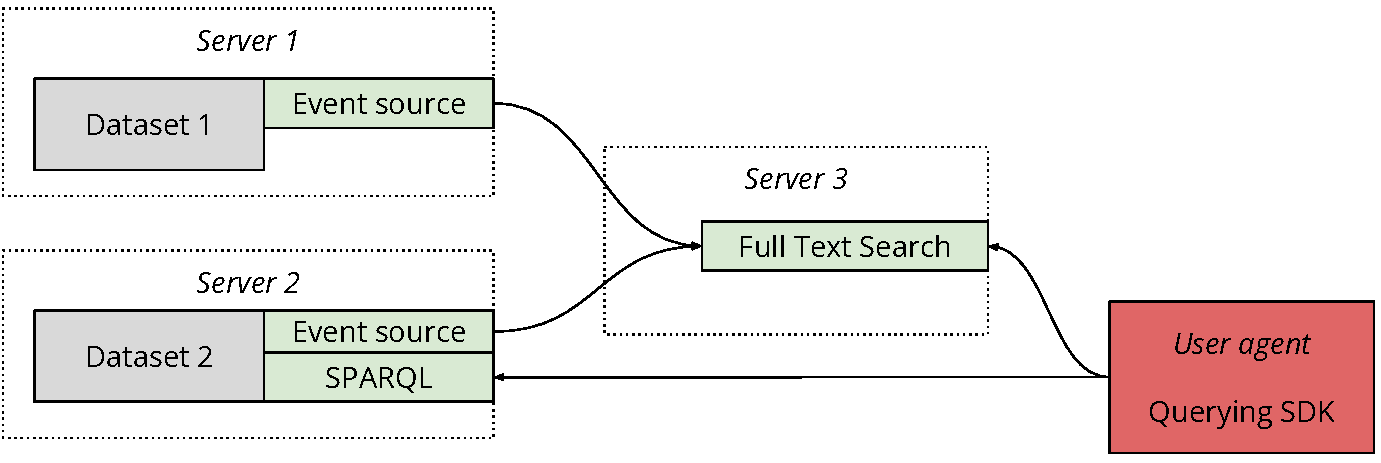
\includegraphics[width=\linewidth]{multiple-views}
  \caption{The same dataset will be published on the Web using multiple interfaces.}
  \label{multiple-views}
\end{figure}

In this paper, we look into making these event sources and derived Web APIs evolvable and preservable, and mitigate the four limitations mentioned above.
Even when a service or dataset is decommissioned, user agents that were once built on top of it, will still be able to resolve queries against archived data.
In \cref{results}, we sketch our first steps into designing the TREE specification for guiding user agents through a fragmented dataset.
In \cref{method}, we then show using a couple of examples how to build what we will call \textit{materializable} Web APIs.
Finally, in the Conclusion\cref{conclusion}, we reiterate the limitations and discuss how these materializable Web APIs tackle them.

\section{State of the art}
\label{sec:sota}
Hartig et al. looked into Link Traversal Query Processing by following the HTTP identifiers it encounters in the triples of Linked Data documents~\cite{hartig2009executing}.
While this works, as also implemented in Comunica\footnote{\url{https://comunica.dev/research/link_traversal/}}~\cite{taelman_iswc_resources_comunica_2018}, it goes too slow for live Web applications in practice, as these data interfaces are not optimized for querying.
In our work, we will look into more directed link traversal, by making the data publishing include explicit hypermedia controls into their results.

Hydra~\cite{lanthaler2013creating} is a domain model introduced in 2013 to bring the power of hypermedia to Linked Data based APIs.
Other work outside the Linked Data domain, such a Hypertext Application Layer (HAL)\footnote{\url{https://apigility.org/documentation/api-primer/halprimer}} and json:api\footnote{\url{https://jsonapi.org/}}, also introduced hypermedia specifications to Web APIs.
In all three of these cases, the hypermedia controls that would afford pruning a client’s search space are limited.
For instance, the nearest concept to the concept of a fragmentation strategy in Hydra\footnote{\url{http://www.hydra-cg.com/spec/latest/core/}} is the concept of a partial collection view\footnote{\url{http://www.hydra-cg.com/spec/latest/core/#collections}}.
This view describes how to get to the first, next, previous or last page.
Yet, no description is provided on whether or not the view is ordered, and thus, when a smart client would visit the page, it would have to iterate across all pages for any query.

Another specification that includes hypermedia controls as part of a broaded protocols is Activity Streams 2.0\footnote{\url{https://www.w3.org/TR/activitystreams-core/}}.
This specification does allow to indicate pages are ordered, yet the description of the ordering itself is left out of scope.
Linked Data Platform (LDP)\footnote{\url{https://www.w3.org/TR/ldp/}} is a World Wide Web (W3C) specification that in an extension also puts forward a paging specification\footnote{\url{https://www.w3.org/TR/ldp-paging/}}.
Despite its conflicts with Hydra and Activity Streams 2.0~\cite{mihindukulasooriyadescribing}, it does put forward a way to describe how a collection is ordered.
It is the only example in the state of the art we found so far that could allow clients to effectively prune their search space to some extent. We did however not find any evidence of clients taking advantage of this specific feature.

In order to enable clients to prune their search space based on hypermedia descriptions beyond simple pagination, we need to come up with a comprehensible specification, as well as describe the client-side algorithm.
An early attempt at making a client detect automatically how to navigate further through a list or things in an ordinal range was with the multidimensional interface specification~\cite{mdi}.

In contrast to the state of the art, we want the specification to describe precisely how the index works, so any client-side query algorithm can benefit without a human developer having to explain how to interpret the responses.

\section{The TREE specification}

We introduce the TREE hypermedia specification to fragment a collection of members in more interesting ways than only simple pagination.
It allows to qualify relations from the current \texttt{tree:Node}---a page or fragment that can be requested using HTTP GET---to multiple other pages, similar to search trees. 
The description allows for a user agent to understand that, when following the link, all members of the collection from that page on will respect a certain condition, such as the fact that the name contains a certain prefix, a value from a literal will be greater or less than a certain value, or is contained in a certain geospatial area.
The full specification can be found in the TREE specification\footnote{\url{https://w3id.org/tree/specification}}.
A concise overview of the specification is depicted in \cref{treespec}.

\begin{figure}
  \centering
  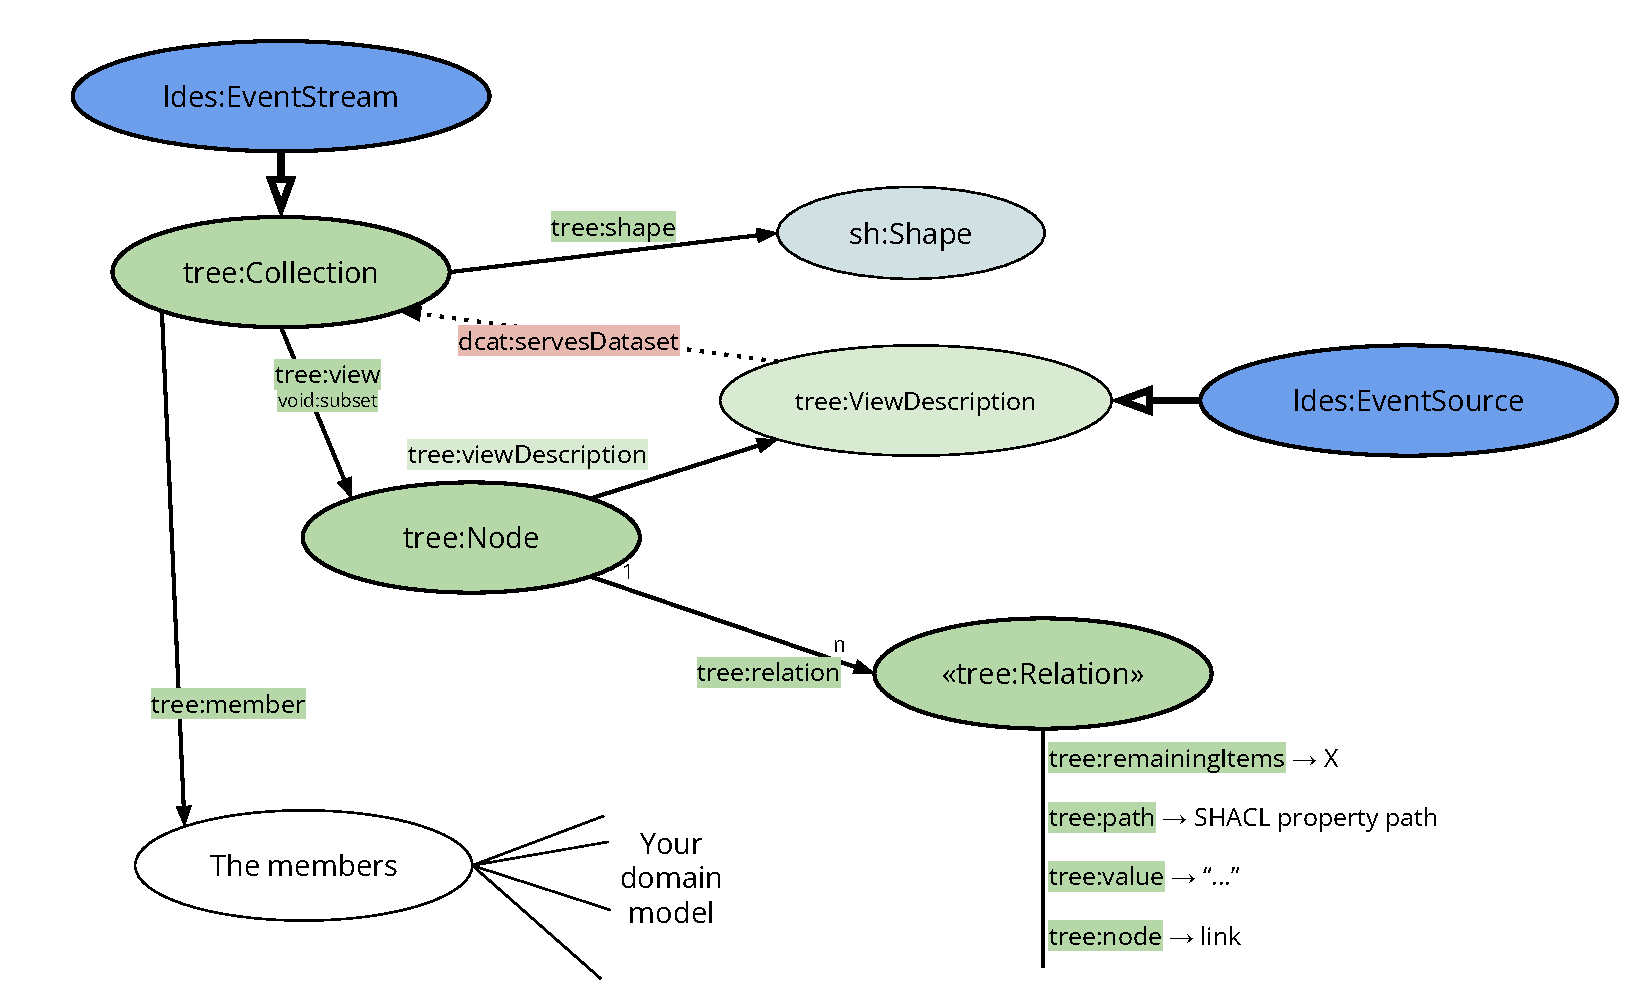
\includegraphics[width=\linewidth]{overview}
  \caption{TREE is a specification to qualify the relation between two pages. It is able to describe to a client whether following a certain page will not be interesting for its current query, and thus whether the client’s search space can be pruned.}
  \label{treespec}
\end{figure}

\subsection{Collection design}

The core collection design is largely inspired by and in line with Hydra.
An instance of a \texttt{tree:Collection} links using the \texttt{tree:member} to the entities it contains.

As a collection will grow too large for one page, a predicate needs to indicate the current page is a subset of the collection, and only one way through which the collection can be viewed.
When all members starting from this \texttt{tree:Node} can be found, the property \texttt{tree:view} can be used, meaning this node can be a starting point for \textit{viewing} all members of the collection.
Otherwise, if not all members can be found from that \texttt{tree:Node}, but if this node also contains a subset of the members in the collection, the property \texttt{void:subset} can be used.

\subsection{Discovery}

A \texttt{tree:Collection} is a subclass of a \texttt{dcat:Dataset}.
The specialization being that it adheres to this collection design.
When a \texttt{tree:Collection} is an ever-growing append-only collection of immutable members, it must be typed using the subclass \texttt{ldes:EventStream}.
A \texttt{tree:Collection}, and its subclasses, should define what their members look like using a SHACL shape\footnote{\url{https://www.w3.org/TR/shacl/}}.
This SHACL shape may prove useful when selecting datasets from a DCAT catalog, also called \textit{dataset discovery}.

However, when there are multiple views defined, a \texttt{tree:ViewDescription} can be defined, which is a subclass of a \texttt{dcat:DataService}.
The specialization being that it describes a Web API on top of a \texttt{tree:Collection}, publishing all members.
If the intention of the view is to publish the event source, the sublass \texttt{ldes:EventSource} can be used as a type.
The type only says something about the intention of the server administrator, and can still contain any kind of structure.
Through the \texttt{tree:ViewDescription}, a user agent can select the right view for the task it has at hand, also called \textit{view discovery}.

The last point in discovery is \textit{interface discovery} to discover the next links to follow from within the view itself.
This is explored in the next subsection on traversing the hypermedia structure.

\subsection{TREE traversal}

We always write TREE with all caps to indicate we take inspiration from traversing search trees, but we cannot guarantee, and do not limit the TREE hypermedia specification to designing search trees.
Even however we would limit it to search trees, counting on the fact that server would not provide you circular references would be incredibly naive.
Therefore, a TREE user agent must always keep a history of nodes it already traversed, and \textit{prune} these nodes from its yet-to-be-visited queue.
Visited nodes may be added again to the queue if the user agent implements a cache invalidation strategy.

The \texttt{tree:Node} describing the current page is linked with the property \texttt{tree:relation} to an entity that is an instance of a subclass of a \texttt{tree:Relation}.
For example, for string search, we have defined the type \texttt{tree:SubstringRelation}.
A \texttt{tree:value} property on top of that relation defines the value to be used in a comparison function defined by the relation, to compare the needs of the user agent with the intention of the relation.
The \texttt{tree:path} describes the property path (using the Shapes Constraints Language (SHACL) Property Paths specification\footnote{\url{https://www.w3.org/TR/shacl/#x2.3.1-shacl-property-paths}}) to be resolved starting from a member, on which this \texttt{tree:value} applies.
Mind that a certain \texttt{tree:Node} can occur multiple times across relations, and that this must be interpretted as a logical AND.
A code example of a relation can be found in \cref{TREE-code-sample}.

Given the list of nodes linked from the pages a user agent already visited, minus these nodes it already visited, it can prune that list further based on the constraints given to the task at hand (e.g., find all members starting with labels starting with the letters \texttt{Ghent}).

\begin{lstlisting}[language=SPARQL,upquote=true,label=TREE-code-sample,caption={A Turtle example of an \texttt{ex:ThisPage} that links to a \texttt{ex:NextPage} through a GreaterThanRelation. A client can assume it must follow the page if its task needs members with a \texttt{sosa:simpleResult} greater than \texttt{5.1234}, to be compared using the double datatype.}]
@prefix tree: <https://w3id.org/tree#>.
@prefix ex: <http://example.org/>.
@prefix xsd: <http://www.w3.org/2001/XMLSchema#>.
@prefix sosa: <http://www.w3.org/ns/sosa/>.

ex:C a tree:Collection ;
    tree:view ex:ThisPage .

ex:ThisPage a tree:Node ;
    tree:relation ex:Relation1 .

ex:Relation1 a tree:GreaterThanRelation ;
    tree:node ex:NextPage ;
    tree:value "5.1234"^^xsd:double ;
    tree:path (sosa:simpleResult) .
\end{lstlisting}


\section{Building materializable interfaces}
\label{sec:method}

The TREE specification allows publishers to construct their own \textbf{materializable hypermedia interfaces}.
We define \textit{a materializable interface} as an interface that has a finite set of URLs that provide an answer.
That way, the interface can be published using a simple file host, but is also very efficient to be hosted through a content delivery network, even if the server itself is built in a dynamic way in which each GET request on a URL potentially triggers a script to be executed.

The strategies in which a dataset can be fragmented is infinite, similar to the amount of indexes one can make on top of a relational database.
One method of thinking about a fragmentation strategy, is \textbf{to only fragment a dataset from the moment a dataset becomes too large for one page}.
The way in which a second page will be added can then be decided based on the needs in the ecosystem.
As illustrated in \cref{multiple-views-2}, the first priority should be to build the relation to the second page based on how the dataset is growing.
That way, that fragmentation can be efficiently used for populating other Web APIs on top of that dataset.
However, when the event source is available, we can optionally support more functionality on top of the dataset

\begin{figure}
  \centering
  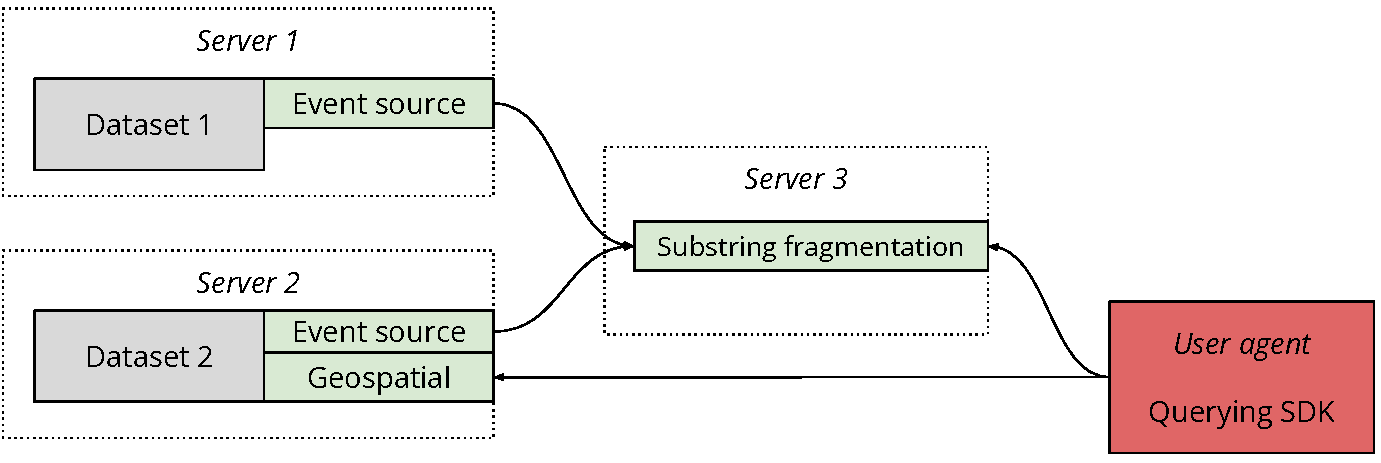
\includegraphics[width=\linewidth]{multiple-views2}
  \caption{A space of materializable interfaces on top of Linked Data interfaces can be queried from the user agents.}
  \label{multiple-views-2}
\end{figure}

The use cases we worked with included querying for geospatial relations, time schedules of public transit data, OpenStreetMap’s road network and taxonomies with text literals such as an address database, geonames, OpenStreetMap names or Wikidata entities.
These cases have been published in their respective papers, for which we provide a concise overview below (as of January 2023).
These use cases describe their search space \texttt{tree:Relation} objects.

\begin{description}
\item[1. Replicating and synchronizing dataset copies across organizations]
A one dimensional pagination of an ever-growing collection of immutable events has interesting caching properties.
Only one page remains to be polled, while all other pages are historic and can be flagged with the \texttt{cache-control: immutable} response header.
In ~\cite{lonneville2021publishing} this is applied on Marine Regions: a gazetteer of standard marine georeference place names and areas. While different organizations build different views on it, all views only need to poll the last page to keep their views in-sync.
In ~\cite{ldes} it is applied on top of both base registries of the Flemish government, as well as a sensor observation stream, proving the method is both useful for
In ~\cite{van2022publishing} it is applied to keep the data from art collections from the city of Ghent in-sync with their digital asset management system and the city’s SPARQL endpoint, through which the history and the current state of the art collections can be queried.
In a similar way, for more fine-grained access to specific windows in time, a B+-tree like fragmentation can also be designed.
 \item[2. Time-based relations for route planning over public transit networks]
Public transit can be modeled as a temporal directed acyclic graph departures and arrivals. With Linked Connections~\cite{rojas2022publishing}, we proposed to fragment this long list of connections from one stop to another in time intervals. A public transit route planner can then perform the route planning algorithm on the infrastructure of the user agent, by selecting the right time window and performing the route planning in a streaming manner, downloading more data when needed.
 \item[3. Geospatial relations for route planning over road and transit networks]
The route planning use case~\cite{delva2019client} illustrates the need for querying with a more open world while retaining query privacy.
By geospatially fragmenting a road network (such as OpenStreetMap), we can select data with a geospatial locality, and/or public transit with a time and geospatial locality.
The public transit data also needs a road network to potentially calculate walks to transfer from one public transit stop to another, and maybe that transfer needs to happen according to the potential constraints of the end-user, whether they are pushing a stroller, in a wheelchair, trained athletes, or visually impaired. However, the profile of user does not need to be leaked to a server in order for the route planning result to be calculated.
 \item[4. Substring-based relations for autocompletion]
Mutatis mutandis for substring autocompletion~\cite{dedecker2021file}: the locality is now not based on geospatial or time-based literals, but on the basis of substring matches with a string literal. Similar benefits can be found.
\end{description}


All these interfaces can be kept in-sync thanks to the event source, but also need to be able to describe how they are derived from which sources.
The result of a workflow over semantically describe streams can already be described~\cite{vercruysse2022describing, guasch2022semantic} by combining LDES, DCAT, SHACL, PROV-O and P-Plan.

\section{Conclusion}

In this paper, although it was already used in previous academic work, we introduced the TREE hypermedia specification for building materializable interfaces.
We chose the term \textit{materializable} as it does not need to be materialized on disk, but it can be as there is only a finite set of HTTP requests that give a result.
Hosting a materializable interface should be possible with almost neglectible hosting costs.
The largest costs should come from the computational power needed to create and update a page from an interface.

This turns the four limitations of more complex query patterns in the introduction into the advantages of materializable interfaces:

\begin{description}
\item[1. You can query your end-user’s world]
Materializable interfaces assume user agents take part in the query evaluation.
That way, it can execute the queries by taking into account data that lives on the user agent’s infrastructure, with access to datasets the end-user has access to. Take for example the use case of route planning: it can take into account their home address, the fact their bike is parked in a certain location, the fact they are in a wheelchair, etc. Personalization can happen without having to build a profile on a remote server.
 \item[2. It becomes possible to archive an interface, not just the data]
 When a server is being decomissioned, an archiving project can traverse the hypermedia links until it replicated all pages to an archive server, and keep the files available and discoverable. That way, even after a server or even publisher disappeared, clients that relied on a certain fragmentation for their functionality can keep on working.
 \item[3. Evolvability can be realized through discovery on multiple levels]
 Different levels of discoverability could be coded against, that wil come with more \textit{evolvability}.
 One idea is to have the start fragment of the specific Web API hardcoded. That way, if the structure of the hypermedia changes, it will always start again from the root of the search space.
 A higher level of evolvability can be achieved when not the URL of the Web API is hardcoded, but the ones of the dataset and a data catalog. That way, through the data catalog, all Web APIs can be discovered that publish the dataset. If one Web API is decommissioned, the user agent can fall back to another Web API publishing the same data. An even higher level of discovery could yet again be achieved by also implementing discovery on the dataset level, to, through the SHACL shape documented with the \texttt{tree:Collection}, and the provenance information attached to it, select these sources that will return an answer to a question.
 \item[4. Queries can be kept private]
The only thing a server sees is that a client is interested in a page of its dataset. It does not see how the query is executed and what the final recommendation or query result provided to the user is. This in stark contrast with Web APIs with URL patterns like \texttt{https://your-domain/weather{?long,lat}} that would be polled for weather information.
\end{description}

\section{Future work}

The current version of the TREE vocabulary has been submitted to LOV~\cite{lov}.
In order to further evolve the specification, we are now starting a TREE/LDES community group at W3C for which we are now seeking support.

The last information on the TREE hypermedia project can be found at \url{https://tree.linkeddatafragments.org}.
In future work, we are also going to tackle graph-based and time series fragmentations with the TREE/LDES method.
Furthermore, the Comunica Querying engine~\cite{taelman_iswc_resources_comunica_2018} is being extended with a TREE hypermedia querying actor that does query planning across multiple hypermedia interfaces.

\begin{acknowledgments}

This work has been support by SolidLab Vlaanderen (Flemish Government, EWI and RRF project V023/10) and the Flemish Smart Data Space (Flemish Government, Digital Flanders and RRF project VV073). The vision on materializable hypermedia interfaces is a result of working with the entire Knowledge on Web-Scale team at Ghent University.

  
\end{acknowledgments}

%%
%% Define the bibliography file to be used
\bibliography{references}

\end{document}

%%
%% End of file
